\documentclass{article}

\usepackage[french]{babel}
\usepackage[utf8]{inputenc}
\usepackage{graphicx}

\title{Todo list : manuel d'utilisation}
\date{\today}
\author{Lucas Franceschino}

\begin{document}
	\maketitle

	\tableofcontents

	\newpage

	\section{Présentation}
	Ce projet est un gestionnaire de tâches écris en Java, dans le cadre de l'UE HLIN505, à la fac de science de Montpellier.\\

	\section{Usage}
	\subsection{Ecran principal}
		Voici l'interface de l'application :\\
		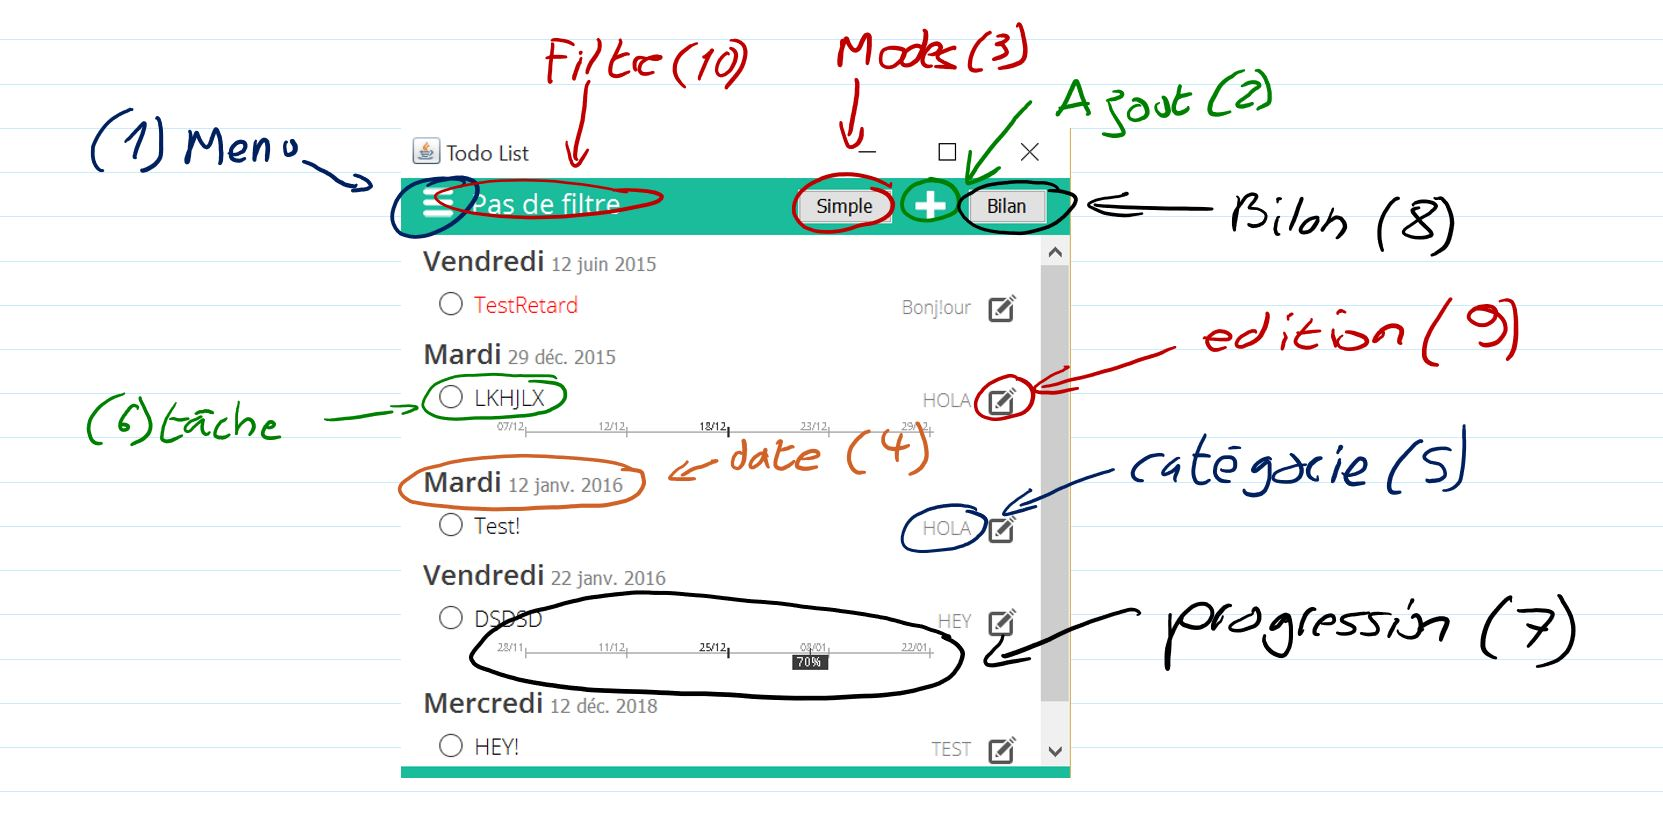
\includegraphics[width=14cm]{images/interface.jpg}
		\begin{enumerate}
			\item \textbf{Le menu} permet d'accéder aux catégories, de les renommer, de les suppimer, d'en ajouter. Aussi, ce menu permet de choisir une catégorie pour filtrer les catégories.
			\item \textbf{Ajout :} pour ajouter une tâche
			\item \textbf{Modes : }3 modes sont possible :
			\begin{itemize}
				\item Simple : les tâches sont affichées par ordre croissant de date d'échéance.
				\item Priorité : les tâches sont affichées par ordre croissant de date d'échéance, en considérant les paliers des dates à long termes comme des dates d'échéances.
				\item Résumé : affiche une tâche importante, trois tâches moyennement importantes, et 5 peu importante.
			\end{itemize} 
			\item \textbf{Date : }une en tête de date regroupe toutes les tâches qui se terminent à cette date.
			\item \textbf{Catégorie : } pour une tâche, il est possible de visualiser dans quelle catégorie celle-ci est, et de l'éditer, en double cliquant dessus, simplement. Après un double clic, le texte se transforme en liste déroulante.
			\item \textbf{Tâche : }on peut voir ici le titre de la tâche, en double cliquant, on peut l'éditer. Pour marquer une tâche comme étant terminée, il suffit de cliquer sur la case à cocher.
			\item \textbf{Progression : }on peut directement voir la progression d'une tâche à long terme par le biais d'un indicateur visuel. En double cliquant sur cet élément visuel, il est possible de modifier le pourcentage de completion de la tâche.
			\item \textbf{Bilan : }permet de générer un bilan paramétré.
			\item \textbf{Edition : }modifie la date d'échéance, et la date de départ si c'est une tâche longue, d'une tâche.
			\item \textbf{Filtres : }visualisation du filtre actuellement appliqué sur la liste des tâches.
		\end{enumerate}
	\subsection{Menu des catégories}
		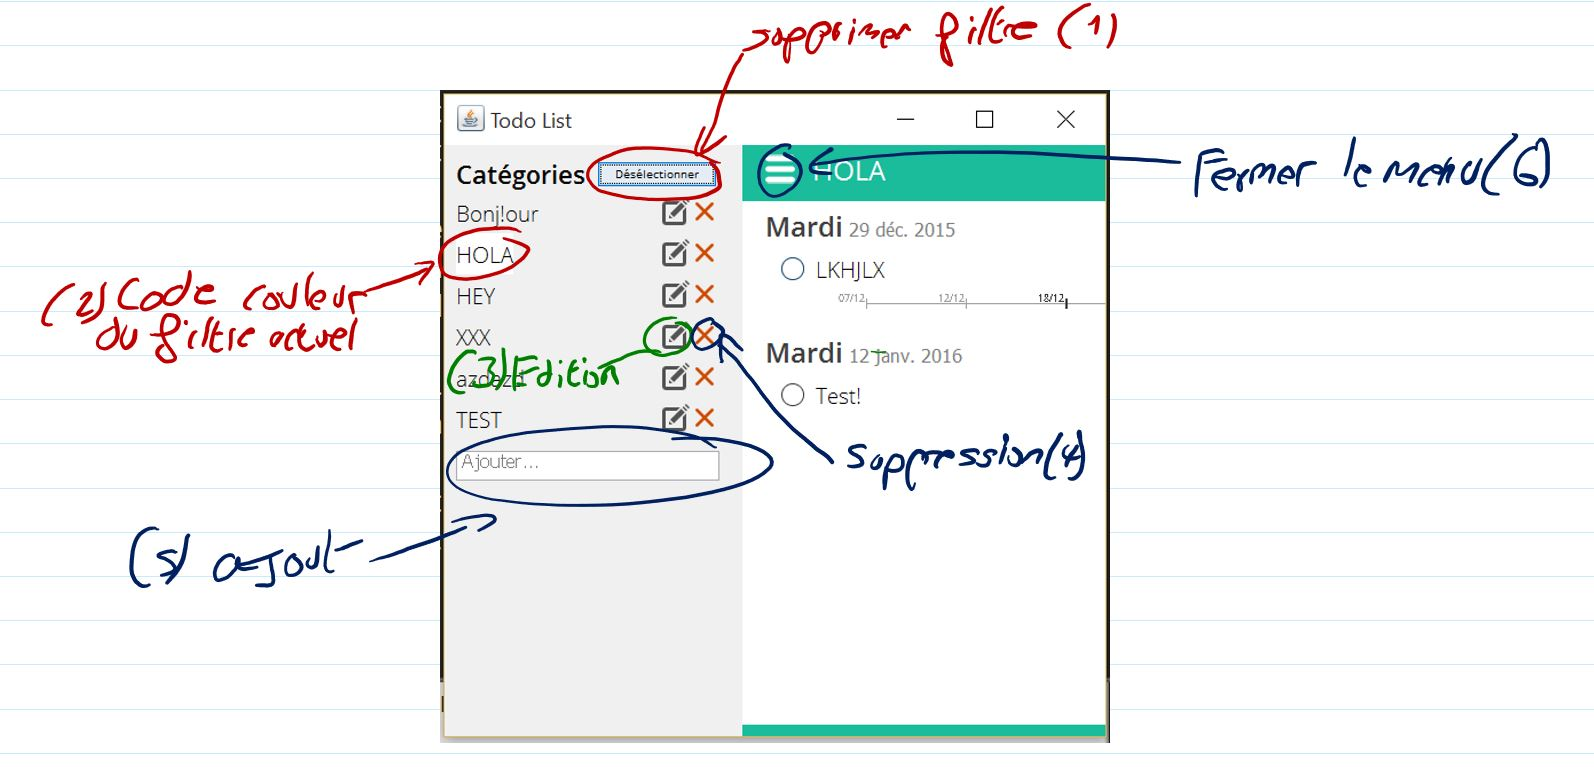
\includegraphics[width=14cm]{images/menu.jpg}
		\begin{enumerate}
			\item \textbf{Supprimer filtre : }le filtre actuel est "HOLA", en cliquant sur ce bouton, on supprime le filtre, et on affiche toute les tâches. Un clic sur ce bouton ferme le menu.
			\item \textbf{Code couleur du filtre actuel : }le filtre actuel est reconnaissable par le biais d'un code couleur : un fond blanc.
			\item \textbf{Etition : }par ce biais on édite une catégorie ;
			\item \textbf{Suppression}
			\item \textbf{Ajout} : tapez un nom de catégorie et appuyez sur entrée et une catégorie sera crée.
			\item \textbf{Fermer le menu} 
		\end{enumerate}
	\subsection{Ajout d'une tâche}
		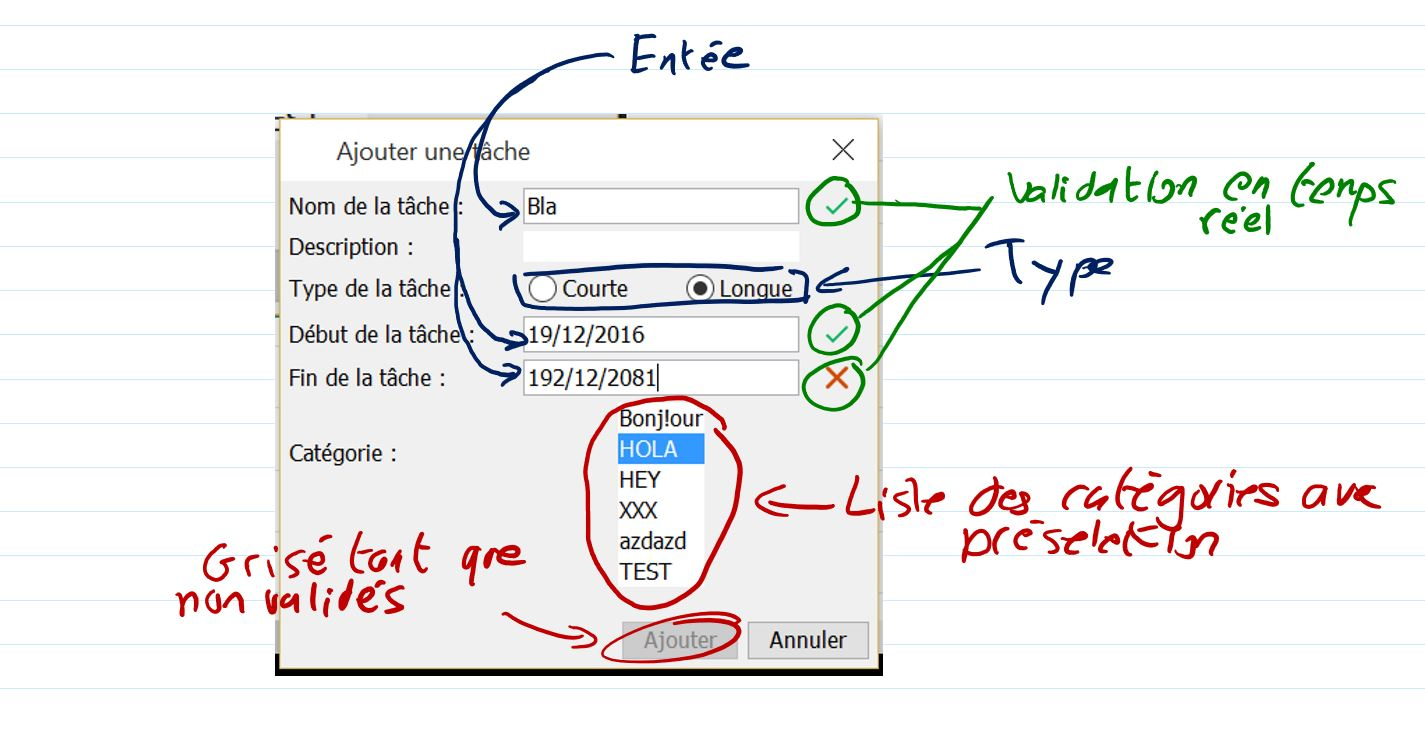
\includegraphics[width=14cm]{images/add.jpg}
	\subsection{Etition d'un bilan}
		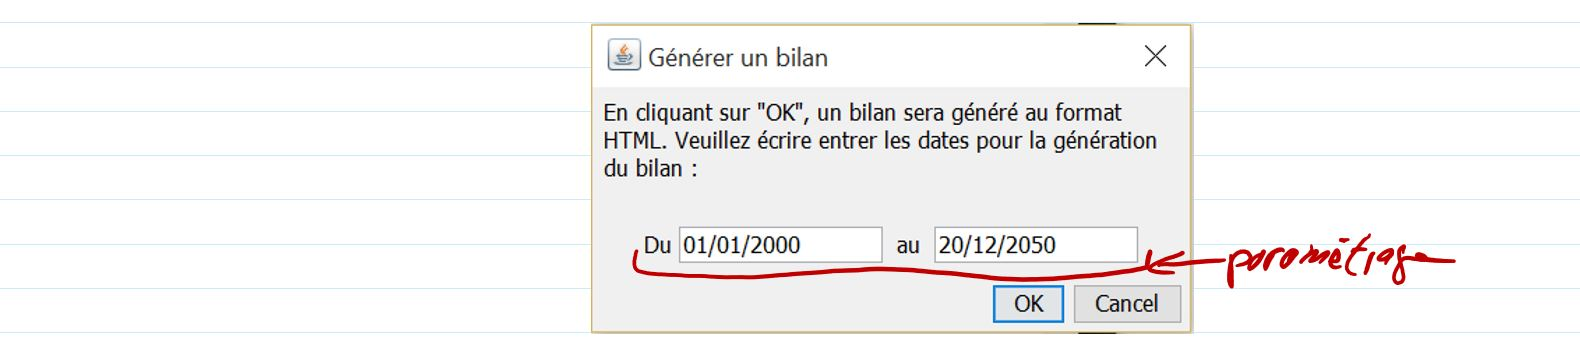
\includegraphics[width=14cm]{images/bilan.jpg}
	\subsection{Supprimer une tâche}
		Il suffit de faire clic droit sur celle-ci, pour voir apparaitre un menu contextuel dédié à cet usage.
\end{document}